%%%%%%%%%%%%%%%%%%%%%%%%%%%%%%%%%%%%%%%%%%%%%%%%%%%%%%%%%%%%%%%%%%%%
%% I, the copyright holder of this work, release this work into the
%% public domain. This applies worldwide. In some countries this may
%% not be legally possible; if so: I grant anyone the right to use
%% this work for any purpose, without any conditions, unless such
%% conditions are required by law.
%%%%%%%%%%%%%%%%%%%%%%%%%%%%%%%%%%%%%%%%%%%%%%%%%%%%%%%%%%%%%%%%%%%%

\documentclass[
  digital,     %% The `digital` option enables the default options for the
               %% digital version of a document. Replace with `printed`
               %% to enable the default options for the printed version
               %% of a document.
%%  color,       %% Uncomment these lines (by removing the %% at the
%%               %% beginning) to use color in the printed version of your
%%               %% document
  oneside,     %% The `oneside` option enables one-sided typesetting,
               %% which is preferred if you are only going to submit a
               %% digital version of your thesis. Replace with `twoside`
               %% for double-sided typesetting if you are planning to
               %% also print your thesis. For double-sided typesetting,
               %% use at least 120 g/m² paper to prevent show-through.
  nosansbold,  %% The `nosansbold` option prevents the use of the
               %% sans-serif type face for bold text. Replace with
               %% `sansbold` to use sans-serif type face for bold text.
  nocolorbold, %% The `nocolorbold` option disables the usage of the
               %% blue color for bold text, instead using black. Replace
               %% with `colorbold` to use blue for bold text.
  lof,         %% The `lof` option prints the List of Figures. Replace
               %% with `nolof` to hide the List of Figures.
  lot,         %% The `lot` option prints the List of Tables. Replace
               %% with `nolot` to hide the List of Tables.
]{fithesis4}
%% The following section sets up the locales used in the thesis.
\usepackage[resetfonts]{cmap} %% We need to load the T2A font encoding
\usepackage[T1,T2A]{fontenc}  %% to use the Cyrillic fonts with Russian texts.
\usepackage[
  main=english, %% By using `czech` or `slovak` as the main locale
                %% instead of `english`, you can typeset the thesis
                %% in either Czech or Slovak, respectively.
  english, german, russian, czech, slovak %% The additional keys allow
]{babel}        %% foreign texts to be typeset as follows:
%%
%%   \begin{otherlanguage}{german}  ... \end{otherlanguage}
%%   \begin{otherlanguage}{russian} ... \end{otherlanguage}
%%   \begin{otherlanguage}{czech}   ... \end{otherlanguage}
%%   \begin{otherlanguage}{slovak}  ... \end{otherlanguage}
%%
%% For non-Latin scripts, it may be necessary to load additional
%% fonts:
\usepackage{paratype}
\def\textrussian#1{{\usefont{T2A}{PTSerif-TLF}{m}{rm}#1}}
%%
%% The following section sets up the metadata of the thesis.
\thesissetup{
    date        = \the\year/\the\month/\the\day,
    university  = mu,
    faculty     = fi,
    type        = bc,
    department  = Department of Computer Systems and Communications,
    author      = Tomáš Zobač,
    gender      = m,
    advisor     = {RNDr. Rudolf Wittner},
    title       = {Implementation of provenance chains traversal},
    TeXtitle    = {Implementation of provenance chains traversal},
    keywords    = {Java, provenance, SOBHA, ÚVT},
    TeXkeywords = {Java, provenance, SOBHA, ÚVT},
    abstract    = {%
      Provenance is a standardized information type that documents the history of an object. It can hold information, such as the origin of an object or previous actions performed on it. This information can be serialized into one of the many supported file formats (e.g., PROVN, XML). These files can then be interconnected, resulting in the creation of a provenance chain. This thesis aims to implement a library for traversing said provenance chains, retrieving information about the precursors or successors of an entity represented in one of the files in the current chain, and optionally retrieving the type of actions performed on the object by the retrieved precursors/successors. The implementation will simulate the operational environment by providing a command-line user interface from where the user can call the mentioned actions on a set of prefactured simulation files. The implementation will follow a W3C PROV-DM standard for provenance notation, and the simulation files will be of a PROVN serialization of provenance data. Additionally to the traversing operations, it will also implement the generation of a provenance metadata to make the simulation of a traversal possible.
    },
    thanks      = {%
      TODO
    },
    bib         = example.bib,
    %% Remove the following line to use the JVS 2018 faculty logo.
    facultyLogo = fithesis-fi,
}
\usepackage{makeidx}      %% The `makeidx` package contains
\makeindex                %% helper commands for index typesetting.
%% These additional packages are used within the document:
\usepackage{paralist} %% Compact list environments
\usepackage{amsmath}  %% Mathematics
\usepackage{amsthm}
\usepackage{amsfonts}
\usepackage{url}      %% Hyperlinks
\usepackage{markdown} %% Lightweight markup
\usepackage{listings} %% Source code highlighting
\lstset{
  basicstyle      = \ttfamily,
  identifierstyle = \color{black},
  keywordstyle    = \color{blue},
  keywordstyle    = {[2]\color{cyan}},
  keywordstyle    = {[3]\color{olive}},
  stringstyle     = \color{teal},
  commentstyle    = \itshape\color{magenta},
  breaklines      = true,
}
\usepackage{floatrow} %% Putting captions above tables
\floatsetup[table]{capposition=top}
\usepackage[babel]{csquotes} %% Context-sensitive quotation marks
\begin{document}
%% The \chapter* command can be used to produce unnumbered chapters:
\chapter*{Introduction}
%% Unlike \chapter, \chapter* does not update the headings and does not
%% enter the chapter to the table of contents. I we want correct
%% headings and a table of contents entry, we must add them manually:
\markright{\textsc{Introduction}}
\addcontentsline{toc}{chapter}{Introduction}

Theses are rumoured to be \enquote{the capstones of education}, so
I decided to write one of my own. If all goes well, I will soon
have a diploma under my belt. Wish me luck!


\chapter{Provenance}
\shorthandoff{-}
Provenance refers to the collective information about the history or origin of something, especially its ownership or location history. It is often used in contexts where it is essential to trace the history of an object, idea, or practice to establish its authenticity, origin, and how it was handled through time. For example, in literature, provenance can relate to the history of a manuscript or a book. Knowing who owned a rare manuscript, where it was kept, and how it was passed down through generations can shed light on its historical importance and authenticity. In the digital realm, provenance refers to the documentation of the history of data, including its origins, processing, and storage. This is important in areas like scientific research, where tracking the origin and modifications of data ensures its reliability and reproducibility. All this information and data mentioned in the examples is collectively called provenance.
\shorthandon{-}

\section{PROV-DM}
\shorthandoff{-}
In order to represent the provenance in a format that can be easily shareable and processable, the W3C PROV-DM (Provenance Data Model) standard was created. The official documentation states, "PROV-DM is the conceptual data model that forms a basis for the W3C provenance (PROV) family of specifications."  PROV-DM is organized into multiple parts called components. The main three components are Entities, Activities, and Agents. Entities hold information about the physical, digital, or other objects, such as the provenance's main subject or other subjects related to it. Activities describe the actions and processes done on or with the entities. As the documentation mentions, "Activities and entities are associated with each other in two different ways: activities utilize entities, and activities produce entities." The last of the main components are Agents, which are responsible for Entities and Activities. In simplified terms, the relation can be imagined as the Agent is the one who did some Activity on an Entity. Relations between these can be tracked thanks to other connecting components such as wasDerivedFrom, wasGeneratedBy, or used. In the end, thanks to the structure of these components, the whole model works as a directed graph.
\shorthandon{-}

\subsection{PROV-N}
\shorthandoff{-}
PROV-N is part of the W3C PROV family of documents for provenance modeling. It is essentially a human-readable textual format for describing the provenance of digital resources. A PROV-N document is a container for provenance descriptions consisting of namespace declarations, expressions, and bundles. It supports extension, allowing for the inclusion of additional attributes and the definition of new expressions. Its content is encoded in UTF-8, which ensures universal readability and accessibility. The main components are distinguished by unique identification, following a QualifiedName notation consisting of a namespace URI, the prefix for easier namespace readability, and the local part. For example, we can look at one of the entities from the used documents.

\begin{verbatim}

entity(ns_surgery:sampleConnector, [
    prov:type='cpm:forwardConnector', 
    cpm:receiverBundleId='ns_pathology:02_scanning.provn', 
    cpm:receiverServiceUri="#URI#"
    ])
    
\end{verbatim}

This entity has an identification of \textit{sampleConnector} with the prefix ns\_surgery and a collection of attributes, where pairs of QualifiedName and Value identify each attribute. The PROV-N documents will be the only ones used in this thesis.
\shorthandon{-}

\section{Provenance chain}
\shorthandoff{-}
The PROV-N documents used in the implementation of this thesis were generated and provided by the thesis supervisor using the "implementation of another thesis". These documents follow a set structure and naming rules described in the standard being developed by the supervisor and his colleagues. Each document contains a single Bundle encompassing all components present. The main structure of the directed graph, created from the bundle's components, consists of three Entity types. The two entry points of the bundle are Entities with types cpm:backwardConnector and cpm:forwardConnector. The backwardConnector points to a forwardConnector with the same identification in the previous bundle. Conversely, the forwardConnector points to a backwardConnector with the same identification in the following bundle. The third Entity has type cpm:currentConnector and points to the current bundle. 

\begin{figure}[htbp]
  \begin{center}
    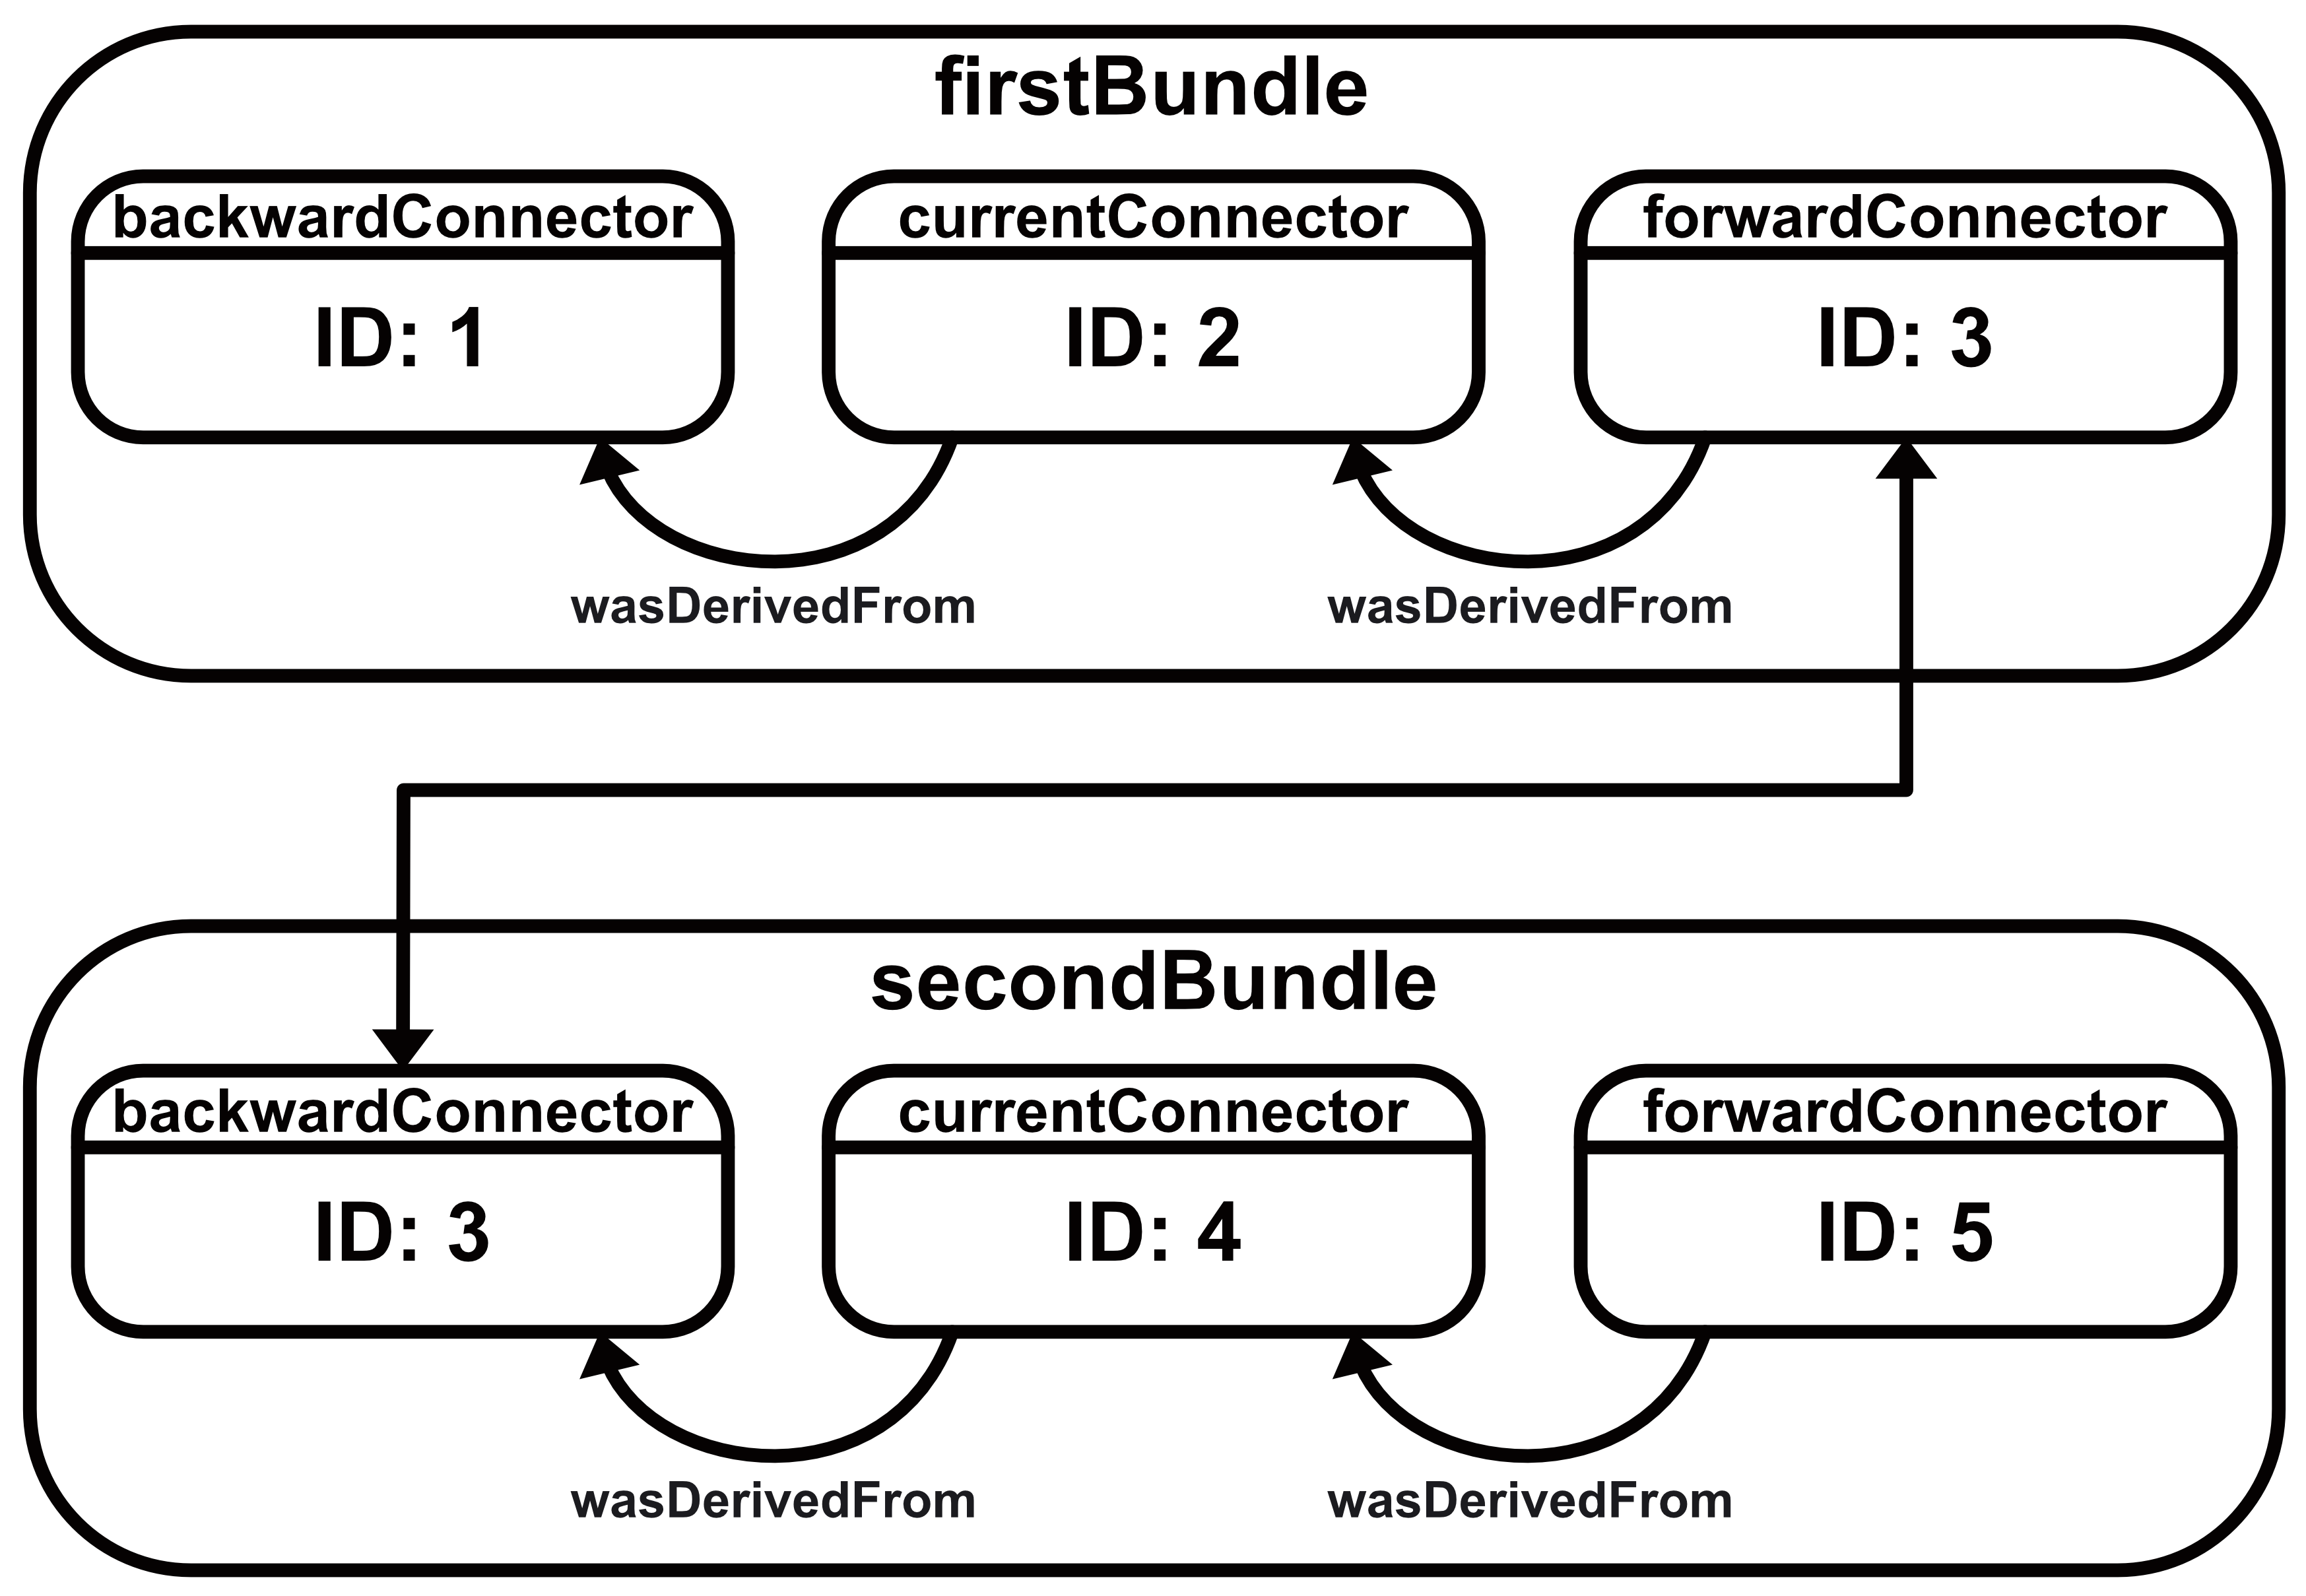
\includegraphics[width=12.5cm]{fithesis/images/bundleconnection.png}
  \end{center}
  \caption{Connection of two provenance bundles}
  \label{fig:bundleconnection}
\end{figure}

 It should be mentioned that this is a simple example, and a single bundle can have multiple connectors of each type pointing to more than one bundle on each side of the traversal.
\shorthandon{-}

\section{Traversing the provenance chain}
\shorthandoff{-}
As mentioned before, the main structure of a bundle consists of three Entities with connector types. These are connected using the wasDerivedFrom statement, effectively creating a traversable path through the bundle. If the target of the traversal is the main Activity of the current bundle, it can be reached using, for example, the wasGeneratedBy or used statement. The same applies to an Agent, which can be reached using the wasAttributedTo statement. As an example, the Figure \ref{fig:bundleexample} is an excerpt from the PROV-N document converted into a graph.

\begin{figure}[htbp]
  \begin{center}
    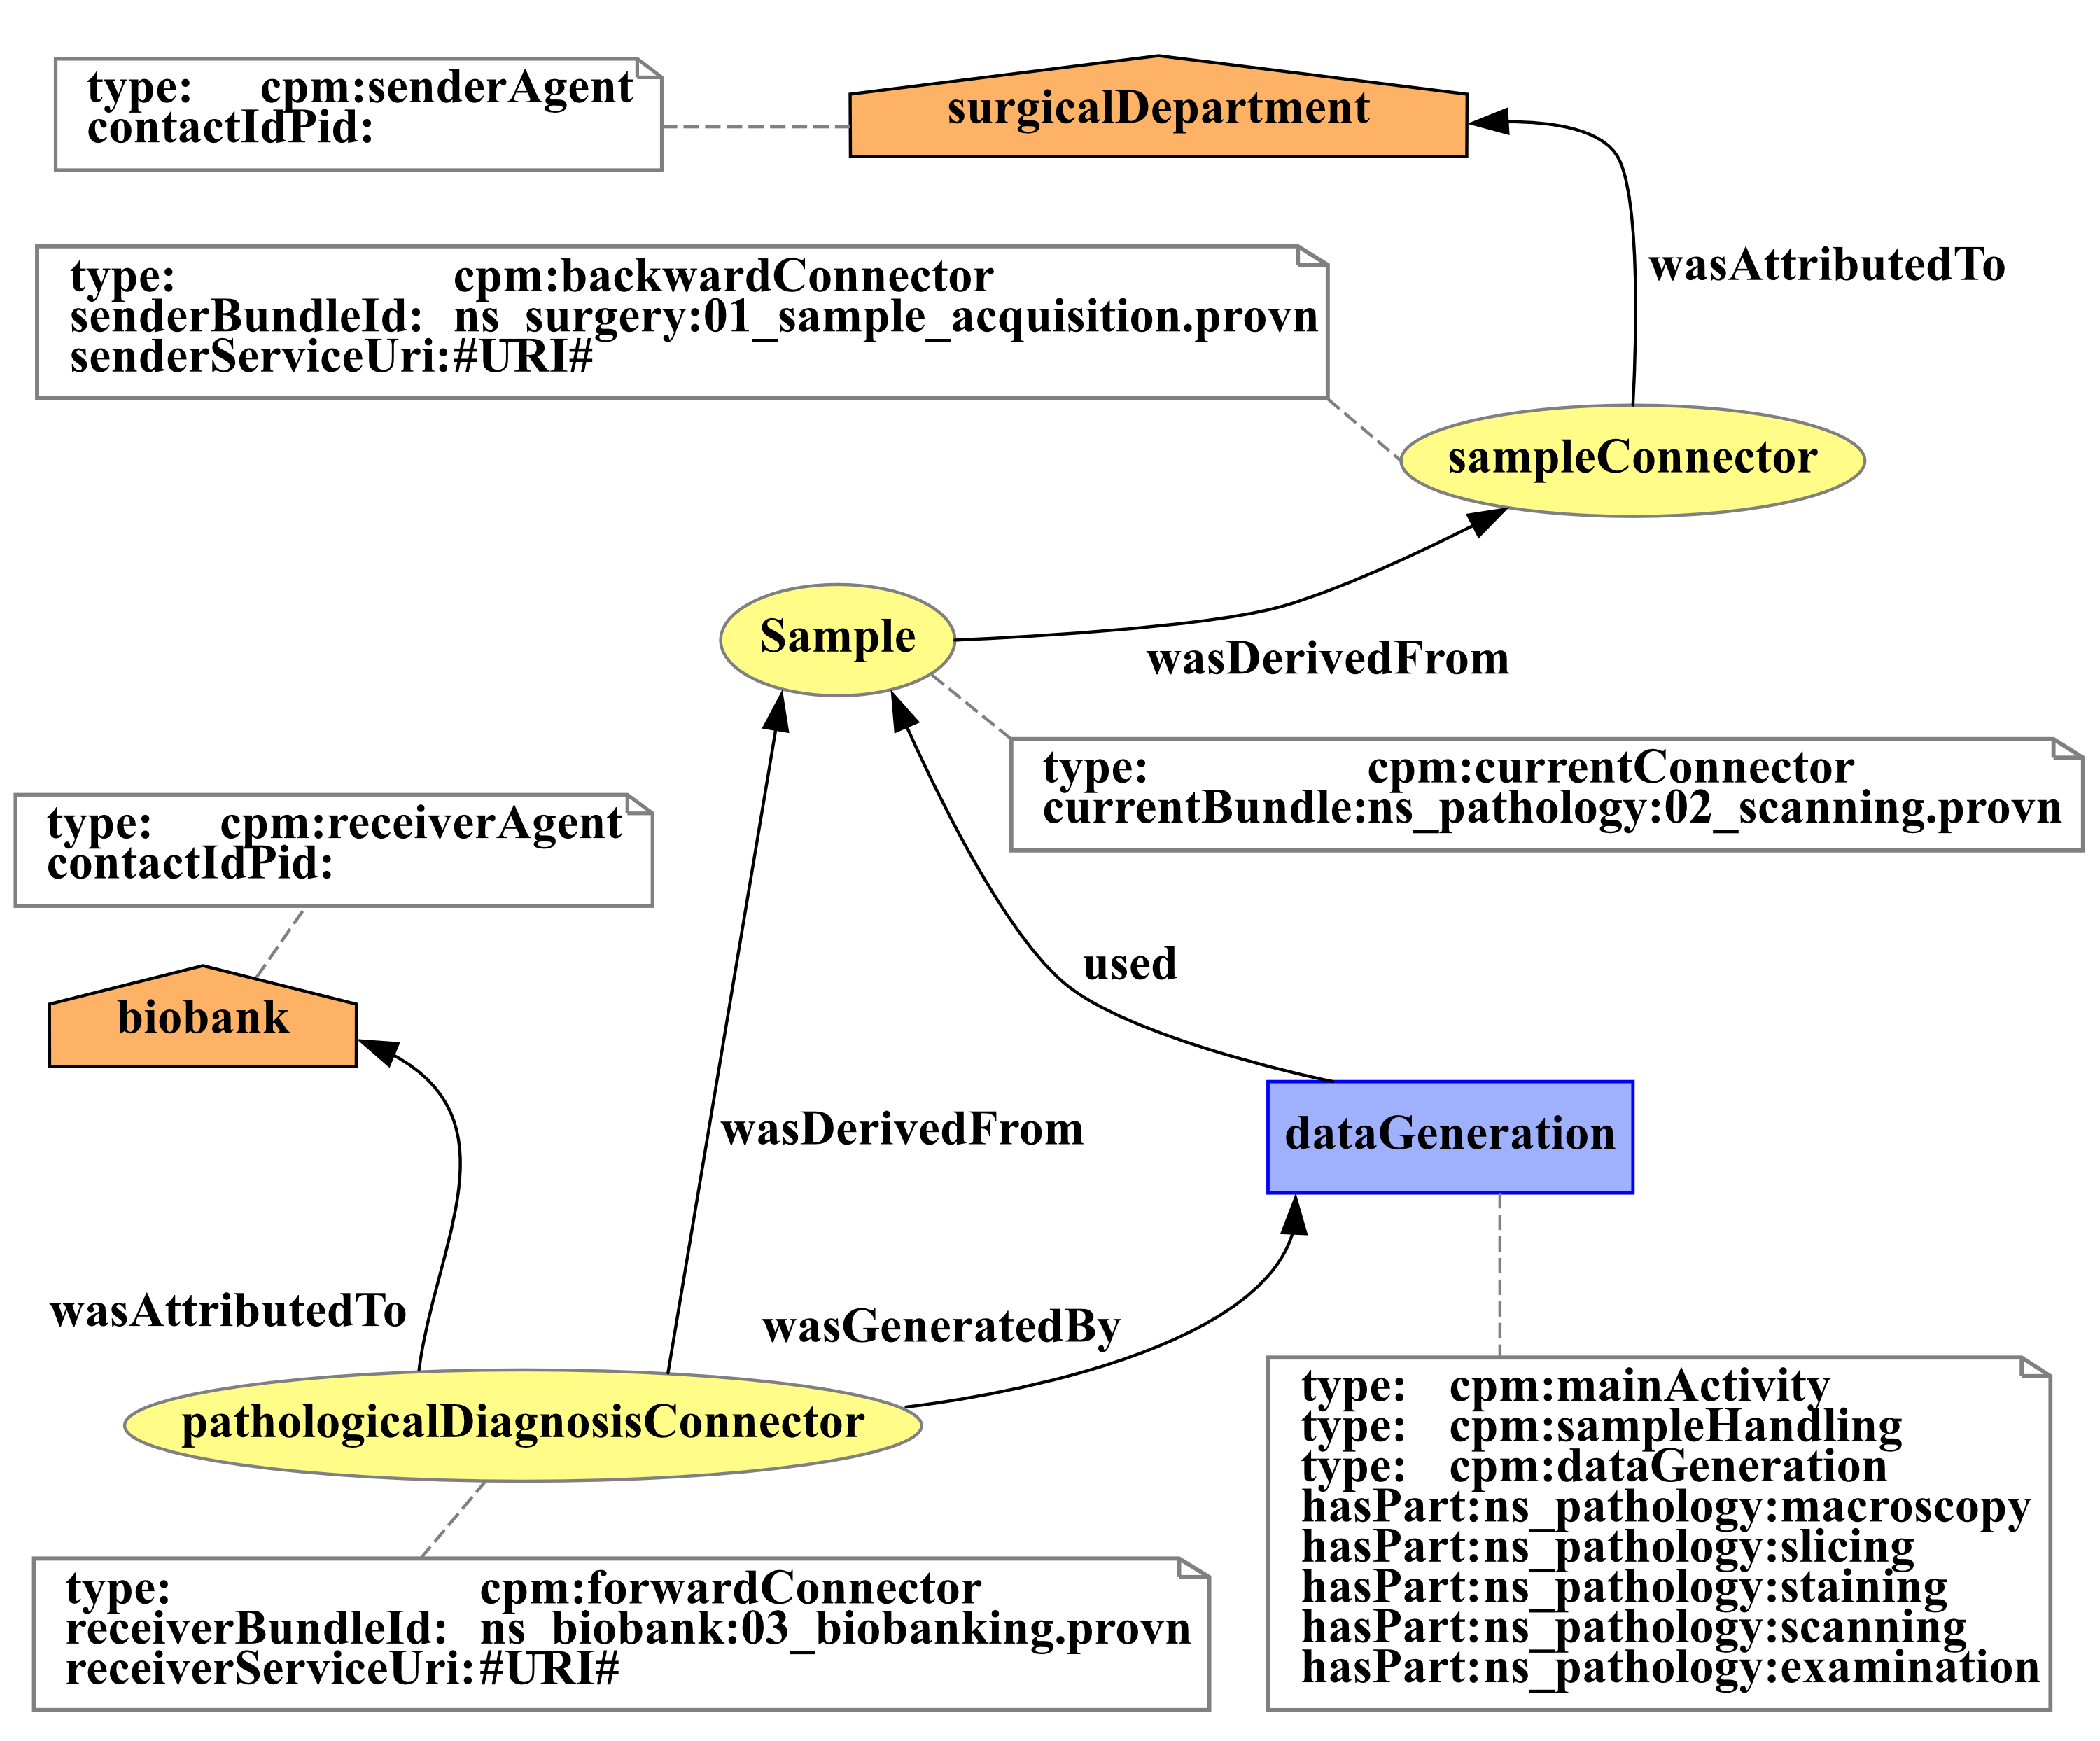
\includegraphics[width=12.7cm]{fithesis/images/examplebigger.png}
  \end{center}
  \caption{Excerpt from a PROV-N document}
  \label{fig:bundleexample}
\end{figure}

The document itself would be structured as follows.

\begin{verbatim}

entity(ns_surgery:sampleConnector,
    [prov:type='cpm:backwardConnector',
    cpm:senderBundleId=
        'ns_surgery:01_sample_acquisition.provn', 
    cpm:senderServiceUri="#URI#"])
entity(ns_pathology:Sample, 
    [prov:type='cpm:currentConnector',
    cpm:currentBundle='ns_pathology:02_scanning.provn'])
entity(ns_pathology:pathologicalDiagnosisConnector, 
    [prov:type='cpm:forwardConnector',
    cpm:receiverBundleId='ns_biobank:03_biobanking.provn', 
    cpm:receiverServiceUri="#URI#"])
agent(ns_pathology:surgicalDepartment, 
    [prov:type='cpm:senderAgent', cpm:contactIdPid=""])
agent(ns_pathology:biobank, 
    [prov:type='cpm:receiverAgent', cpm:contactIdPid=""])
activity(ns_pathology:dataGeneration, -, -, 
    [prov:type=
        'cpm:mainActivity', prov:type='cpm:sampleHandling',
    prov:type='cpm:dataGeneration', 
    dct:hasPart='ns_pathology:macroscopy', 
    dct:hasPart='ns_pathology:slicing',
    dct:hasPart='ns_pathology:staining', 
    dct:hasPart='ns_pathology:scanning',
    dct:hasPart='ns_pathology:examination'])
wasDerivedFrom(ns_pathology:Sample, 
    ns_surgery:sampleConnector, -, -, -)
wasDerivedFrom(ns_pathology:pathologicalDiagnosisConnector, 
    ns_pathology:Sample, -, -, -)
wasAttributedTo(ns_surgery:sampleConnector, 
    ns_pathology:surgicalDepartment)
wasAttributedTo(ns_pathology:pathologicalDiagnosisConnector, 
    ns_pathology:biobank)
wasGeneratedBy(ns_pathology:pathologicalDiagnosisConnector, 
    ns_pathology:dataGeneration, -)
used(ns_pathology:dataGeneration, ns_pathology:Sample, -)
    
\end{verbatim}

Considering we arrived from the bundle 01\verb|_|sample\verb|_|acquisition, the next step would be to use a wasDerivedFrom statement where the backwardConnector is in the role of a used Entity. 

\begin{verbatim}

cpm:senderBundleId=
    'ns_surgery:01_sample_acquisition.provn'

entity(ns_surgery:sampleConnector,
    [prov:type='cpm:backwardConnector',
    cpm:senderBundleId=
        'ns_surgery:01_sample_acquisition.provn', 
    cpm:senderServiceUri="#URI#"])

wasDerivedFrom(ns_pathology:Sample, 
    ns_surgery:sampleConnector, -, -, -)
    
\end{verbatim}

After moving to the currentConnector, the process can be either repeated or using the used statement, the main Activity of the current bundle can be accessed.\\\\Proceed: 
\begin{verbatim}
entity(ns_pathology:Sample, 
    [prov:type='cpm:currentConnector',
    cpm:currentBundle='ns_pathology:02_scanning.provn'])

wasDerivedFrom(ns_pathology:pathologicalDiagnosisConnector, 
    ns_pathology:Sample, -, -, -)
    
\end{verbatim}
Retrieve Activity:
\begin{verbatim}
entity(ns_pathology:Sample, 
    [prov:type='cpm:currentConnector',
    cpm:currentBundle='ns_pathology:02_scanning.provn'])

used(ns_pathology:dataGeneration, ns_pathology:Sample, -)

activity(ns_pathology:dataGeneration, -, -, 
    [prov:type=
        'cpm:mainActivity', prov:type='cpm:sampleHandling',
    prov:type='cpm:dataGeneration', 
    dct:hasPart='ns_pathology:macroscopy', 
    dct:hasPart='ns_pathology:slicing',
    dct:hasPart='ns_pathology:staining', 
    dct:hasPart='ns_pathology:scanning',
    dct:hasPart='ns_pathology:examination'])
    
\end{verbatim}

After reaching the end of the bundle's graph, we can enter another bundle by looking into the attributes of the forwardConnector to find where it is pointing (also seen in the Figure \ref{fig:bundleconnection}).

\begin{verbatim}

entity(ns_pathology:pathologicalDiagnosisConnector, 
    [prov:type='cpm:forwardConnector',
    cpm:receiverBundleId='ns_biobank:03_biobanking.provn', 
    cpm:receiverServiceUri="#URI#"])

cpm:receiverBundleId='ns_biobank:03_biobanking.provn'
    
\end{verbatim}

\shorthandon{-}


\chapter{Planning}
\section{Java and Python library differences}
Lorem ipsum dolor sit amet, consectetur adipiscing elit. Integer finibus commodo leo. Nullam blandit imperdiet magna, sit amet tempor tortor sagittis vitae. Lorem ipsum dolor sit amet, consectetur adipiscing elit. Cras elementum diam vel eros tristique, at maximus tortor ultricies.

\section{Drafting}
Lorem ipsum dolor sit amet, consectetur adipiscing elit. Integer finibus commodo leo. Nullam blandit imperdiet magna, sit amet tempor tortor sagittis vitae. Lorem ipsum dolor sit amet, consectetur adipiscing elit. Cras elementum diam vel eros tristique, at maximus tortor ultricies.


\chapter{Implementation}
\section{Used technologies}
\shorthandoff{-}
\subsection{ProvToolBox}
Lorem ipsum dolor sit amet, consectetur adipiscing elit. Integer finibus commodo leo. Nullam blandit imperdiet magna, sit amet tempor tortor sagittis vitae. Lorem ipsum dolor sit amet, consectetur adipiscing elit. Cras elementum diam vel eros tristique, at maximus tortor ultricies.

\subsubsection{PROV MODEL}
Lorem ipsum dolor sit amet, consectetur adipiscing elit. Integer finibus commodo leo. Nullam blandit imperdiet magna, sit amet tempor tortor sagittis vitae. Lorem ipsum dolor sit amet, consectetur adipiscing elit. Cras elementum diam vel eros tristique, at maximus tortor ultricies.

\subsubsection{PROV INTEROP: LIGHT}
Lorem ipsum dolor sit amet, consectetur adipiscing elit. Integer finibus commodo leo. Nullam blandit imperdiet magna, sit amet tempor tortor sagittis vitae. Lorem ipsum dolor sit amet, consectetur adipiscing elit. Cras elementum diam vel eros tristique, at maximus tortor ultricies.

\subsection{Jackson Databind}
Lorem ipsum dolor sit amet, consectetur adipiscing elit. Integer finibus commodo leo. Nullam blandit imperdiet magna, sit amet tempor tortor sagittis vitae. Lorem ipsum dolor sit amet, consectetur adipiscing elit. Cras elementum diam vel eros tristique, at maximus tortor ultricies.

\subsection{GitLab4J API}
Lorem ipsum dolor sit amet, consectetur adipiscing elit. Integer finibus commodo leo. Nullam blandit imperdiet magna, sit amet tempor tortor sagittis vitae. Lorem ipsum dolor sit amet, consectetur adipiscing elit. Cras elementum diam vel eros tristique, at maximus tortor ultricies.

\subsection{JLine Bundle}
Lorem ipsum dolor sit amet, consectetur adipiscing elit. Integer finibus commodo leo. Nullam blandit imperdiet magna, sit amet tempor tortor sagittis vitae. Lorem ipsum dolor sit amet, consectetur adipiscing elit. Cras elementum diam vel eros tristique, at maximus tortor ultricies.

\subsection{Jansi}
Lorem ipsum dolor sit amet, consectetur adipiscing elit. Integer finibus commodo leo. Nullam blandit imperdiet magna, sit amet tempor tortor sagittis vitae. Lorem ipsum dolor sit amet, consectetur adipiscing elit. Cras elementum diam vel eros tristique, at maximus tortor ultricies.

\subsection{Apache Maven Shade Plugin}
Lorem ipsum dolor sit amet, consectetur adipiscing elit. Integer finibus commodo leo. Nullam blandit imperdiet magna, sit amet tempor tortor sagittis vitae. Lorem ipsum dolor sit amet, consectetur adipiscing elit. Cras elementum diam vel eros tristique, at maximus tortor ultricies.
\shorthandon{-}

\section{Components}
Lorem ipsum dolor sit amet, consectetur adipiscing elit. Integer finibus commodo leo. Nullam blandit imperdiet magna, sit amet tempor tortor sagittis vitae. Lorem ipsum dolor sit amet, consectetur adipiscing elit. Cras elementum diam vel eros tristique, at maximus tortor ultricies. Curabitur urna magna, dictum at porta rutrum, congue nec justo. Nam ac rhoncus lectus. Ut feugiat volutpat ornare. Mauris quis neque nec lorem vestibulum iaculis. Proin posuere nisi eget nisi tristique, eu tempus nibh ultricies.

Nunc sagittis id purus quis facilisis. Etiam ullamcorper massa ut justo volutpat, quis malesuada lectus fermentum. Maecenas orci augue, dictum vel risus ut, finibus tincidunt magna. Praesent semper vehicula nulla, eu dignissim elit aliquet in. Mauris ultricies tortor sed justo congue, eu pretium sapien egestas. Aliquam erat volutpat. Duis elementum urna nec felis pharetra, egestas aliquam turpis aliquam. Donec commodo, felis vitae pulvinar interdum, nisl felis feugiat est, vel dictum augue lacus nec elit. Etiam a cursus ligula. Sed luctus nisl at rhoncus ullamcorper. Suspendisse vitae sapien porttitor, auctor quam ac, volutpat tellus. Phasellus cursus, enim vel tristique porttitor, velit dolor viverra sapien, eu lacinia elit erat cursus augue. Fusce sodales venenatis lacus, eget rutrum lorem bibendum vel.

\section{Simulation}
Lorem ipsum dolor sit amet, consectetur adipiscing elit. Integer finibus commodo leo. Nullam blandit imperdiet magna, sit amet tempor tortor sagittis vitae. Lorem ipsum dolor sit amet, consectetur adipiscing elit. Cras elementum diam vel eros tristique, at maximus tortor ultricies. Curabitur urna magna, dictum at porta rutrum, congue nec justo. Nam ac rhoncus lectus. Ut feugiat volutpat ornare. Mauris quis neque nec lorem vestibulum iaculis. Proin posuere nisi eget nisi tristique, eu tempus nibh ultricies.

Nunc sagittis id purus quis facilisis. Etiam ullamcorper massa ut justo volutpat, quis malesuada lectus fermentum. Maecenas orci augue, dictum vel risus ut, finibus tincidunt magna. Praesent semper vehicula nulla, eu dignissim elit aliquet in. Mauris ultricies tortor sed justo congue, eu pretium sapien egestas. Aliquam erat volutpat. Duis elementum urna nec felis pharetra, egestas aliquam turpis aliquam. Donec commodo, felis vitae pulvinar interdum, nisl felis feugiat est, vel dictum augue lacus nec elit. Etiam a cursus ligula. Sed luctus nisl at rhoncus ullamcorper. Suspendisse vitae sapien porttitor, auctor quam ac, volutpat tellus. Phasellus cursus, enim vel tristique porttitor, velit dolor viverra sapien, eu lacinia elit erat cursus augue. Fusce sodales venenatis lacus, eget rutrum lorem bibendum vel.

\section{Algorithm}
Lorem ipsum dolor sit amet, consectetur adipiscing elit. Integer finibus commodo leo. Nullam blandit imperdiet magna, sit amet tempor tortor sagittis vitae. Lorem ipsum dolor sit amet, consectetur adipiscing elit. Cras elementum diam vel eros tristique, at maximus tortor ultricies. Curabitur urna magna, dictum at porta rutrum, congue nec justo. Nam ac rhoncus lectus. Ut feugiat volutpat ornare. Mauris quis neque nec lorem vestibulum iaculis. Proin posuere nisi eget nisi tristique, eu tempus nibh ultricies.

Nunc sagittis id purus quis facilisis. Etiam ullamcorper massa ut justo volutpat, quis malesuada lectus fermentum. Maecenas orci augue, dictum vel risus ut, finibus tincidunt magna. Praesent semper vehicula nulla, eu dignissim elit aliquet in. Mauris ultricies tortor sed justo congue, eu pretium sapien egestas. Aliquam erat volutpat. Duis elementum urna nec felis pharetra, egestas aliquam turpis aliquam. Donec commodo, felis vitae pulvinar interdum, nisl felis feugiat est, vel dictum augue lacus nec elit. Etiam a cursus ligula. Sed luctus nisl at rhoncus ullamcorper. Suspendisse vitae sapien porttitor, auctor quam ac, volutpat tellus. Phasellus cursus, enim vel tristique porttitor, velit dolor viverra sapien, eu lacinia elit erat cursus augue. Fusce sodales venenatis lacus, eget rutrum lorem bibendum vel.

\section{Deployment}
Lorem ipsum dolor sit amet, consectetur adipiscing elit. Integer finibus commodo leo. Nullam blandit imperdiet magna, sit amet tempor tortor sagittis vitae. Lorem ipsum dolor sit amet, consectetur adipiscing elit. Cras elementum diam vel eros tristique, at maximus tortor ultricies. Curabitur urna magna, dictum at porta rutrum, congue nec justo. Nam ac rhoncus lectus. Ut feugiat volutpat ornare. Mauris quis neque nec lorem vestibulum iaculis. Proin posuere nisi eget nisi tristique, eu tempus nibh ultricies.

Nunc sagittis id purus quis facilisis. Etiam ullamcorper massa ut justo volutpat, quis malesuada lectus fermentum. Maecenas orci augue, dictum vel risus ut, finibus tincidunt magna. Praesent semper vehicula nulla, eu dignissim elit aliquet in. Mauris ultricies tortor sed justo congue, eu pretium sapien egestas. Aliquam erat volutpat. Duis elementum urna nec felis pharetra, egestas aliquam turpis aliquam. Donec commodo, felis vitae pulvinar interdum, nisl felis feugiat est, vel dictum augue lacus nec elit. Etiam a cursus ligula. Sed luctus nisl at rhoncus ullamcorper. Suspendisse vitae sapien porttitor, auctor quam ac, volutpat tellus. Phasellus cursus, enim vel tristique porttitor, velit dolor viverra sapien, eu lacinia elit erat cursus augue. Fusce sodales venenatis lacus, eget rutrum lorem bibendum vel.


\chapter{Manual}
\shorthandoff{-}
\section{Set-up}
To utilize the library, it is necessary to have Maven and Java properly configured. To simplify the process for users, the implementation is currently spread across multiple Git repositories, including two on FI and ICS GitLab sites and one on the author's personal GitHub page. To obtain the library, clone the repository or use the download button to retrieve the entire repository bundled in a zip or another archive file.

\subsection{Retrieving the repository}
In order to clone a repository, it is important to confirm that Git is installed on the device. Following this, proceed to the repository's page on GitLab or GitHub and locate the "Clone" button. A URL to copy will be generated by clicking on this button. Next, launch the terminal or command prompt, navigate to the directory where the repository should be stored, and execute the command 'git clone [URL]', replacing [URL] with the URL you copied earlier. Doing this will generate a local copy of the repository on the device. If cloning is not possible, an alternative is to download the repository as a ZIP file. On the repository's page, look for the "Download ZIP" option, typically found in the same section as the clone option. Clicking on this will download the repository's contents in a compressed file, which can then be extracted to the preferred location.

\subsection{Simulating the environment}
The initiation of simulation files is the first step in simulating an environment, which requires the retrieval of specific files necessary for the simulated environment to function effectively. To achieve this, the cloned repository should be opened in the console. The submodule can be navigated by using the command.

\begin{verbatim}
$ cd. \src\main\resources\bthesis-provenancechain-digpat  
\end{verbatim}

Once the submodule is reached, the command 

\begin{verbatim}
$ git submodule foreach git fetch –tags
\end{verbatim}

should be executed. After it finishes, there should be no output. Finally, the command

\begin{verbatim}
$ git submodule update --init --recursive  
\end{verbatim}

should be run to conclude the process. This will ensure that the bthesis-provenancechain-digpat submodule contains the required .provn files.

\section{Building}
The jar file is packaged using the Maven Shade plugin, which is the preferred method. To create the jar file, navigate to the cloned repository using the console and run the \textbf{\texttt{'mvn clean package'}} command. After creating the jar file, it can be launched by executing the command \textbf{\texttt{'java -jar }\path{.\target\BThesis-ProvenanceChain-VERSION-shaded.jar'}}. In the event that the intended environment does not have a JRE, the \textbf{\texttt{'jpackage'}} command line tool provided by Java can be used to create a platform-specific installer.

\section{Omitting the simulated environment}
To facilitate traversal simulation, the implementation employs several classes and files that provide the necessary objects for the algorithm to function. These classes have been transferred to packages labeled 'bthesis.provenancechain.simulation' and 'bthesis.metageneration' to enhance clarity. At the same time, the required files reside in the previously mentioned submodule 'src.main.resources.bthesis-provenancechain-digpat'. However, these components can be omitted if the required classes are adequately substituted.
\shorthandon{-}


\chapter*{Conclusion}
\markright{\textsc{Conclusion}}
\addcontentsline{toc}{chapter}{Conclusion}
\shorthandoff{-}
Lorem ipsum dolor sit amet, consectetur adipiscing elit. Integer finibus commodo leo. Nullam blandit imperdiet magna, sit amet tempor tortor sagittis vitae. Lorem ipsum dolor sit amet, consectetur adipiscing elit. Cras elementum diam vel eros tristique, at maximus tortor ultricies. Curabitur urna magna, dictum at porta rutrum, congue nec justo. Nam ac rhoncus lectus. Ut feugiat volutpat ornare. Mauris quis neque nec lorem vestibulum iaculis. Proin posuere nisi eget nisi tristique, eu tempus nibh ultricies.
\shorthandon{-}

After linking a bibliography data\-base files to the document using
the \verb"\"\texttt{thesis\discretionary{-}{}{}setup\{bib\discretionary{=}{=}{=}%
\{\textit{file1},\textit{file2},\,\ldots\,\}\}} command, you can
start citing the entries. This is just dummy text
\parencite{borgman03} lightly sprinkled with citations
\parencite[p.~123]{greenberg98}. Several sources can be cited at
once: \cite{borgman03,greenberg98,thanh01}.
\citetitle{greenberg98} was written by \citeauthor{greenberg98} in
\citeyear{greenberg98}. We can also produce \textcite{greenberg98}%
\ or %% Let us define a compound command:
\def\citeauthoryear#1{(\textcite{#1},~\citeyear{#1})}%
\citeauthoryear{greenberg98}%
. The full bibliographic citation is:
\emph{\fullcite{greenberg98}}. We can easily insert a bibliographic
citation into the footnote\footfullcite{greenberg98}.

\printbibliography[heading=bibintoc]

\end{document}
